% This file was created by matlab2tikz.
%
\definecolor{mycolor1}{rgb}{0.05882,0.83922,0.63529}%
\definecolor{mycolor2}{rgb}{0.12941,0.12941,0.12941}%
\definecolor{mycolor3}{rgb}{0.05882,0.61961,0.83529}%
%
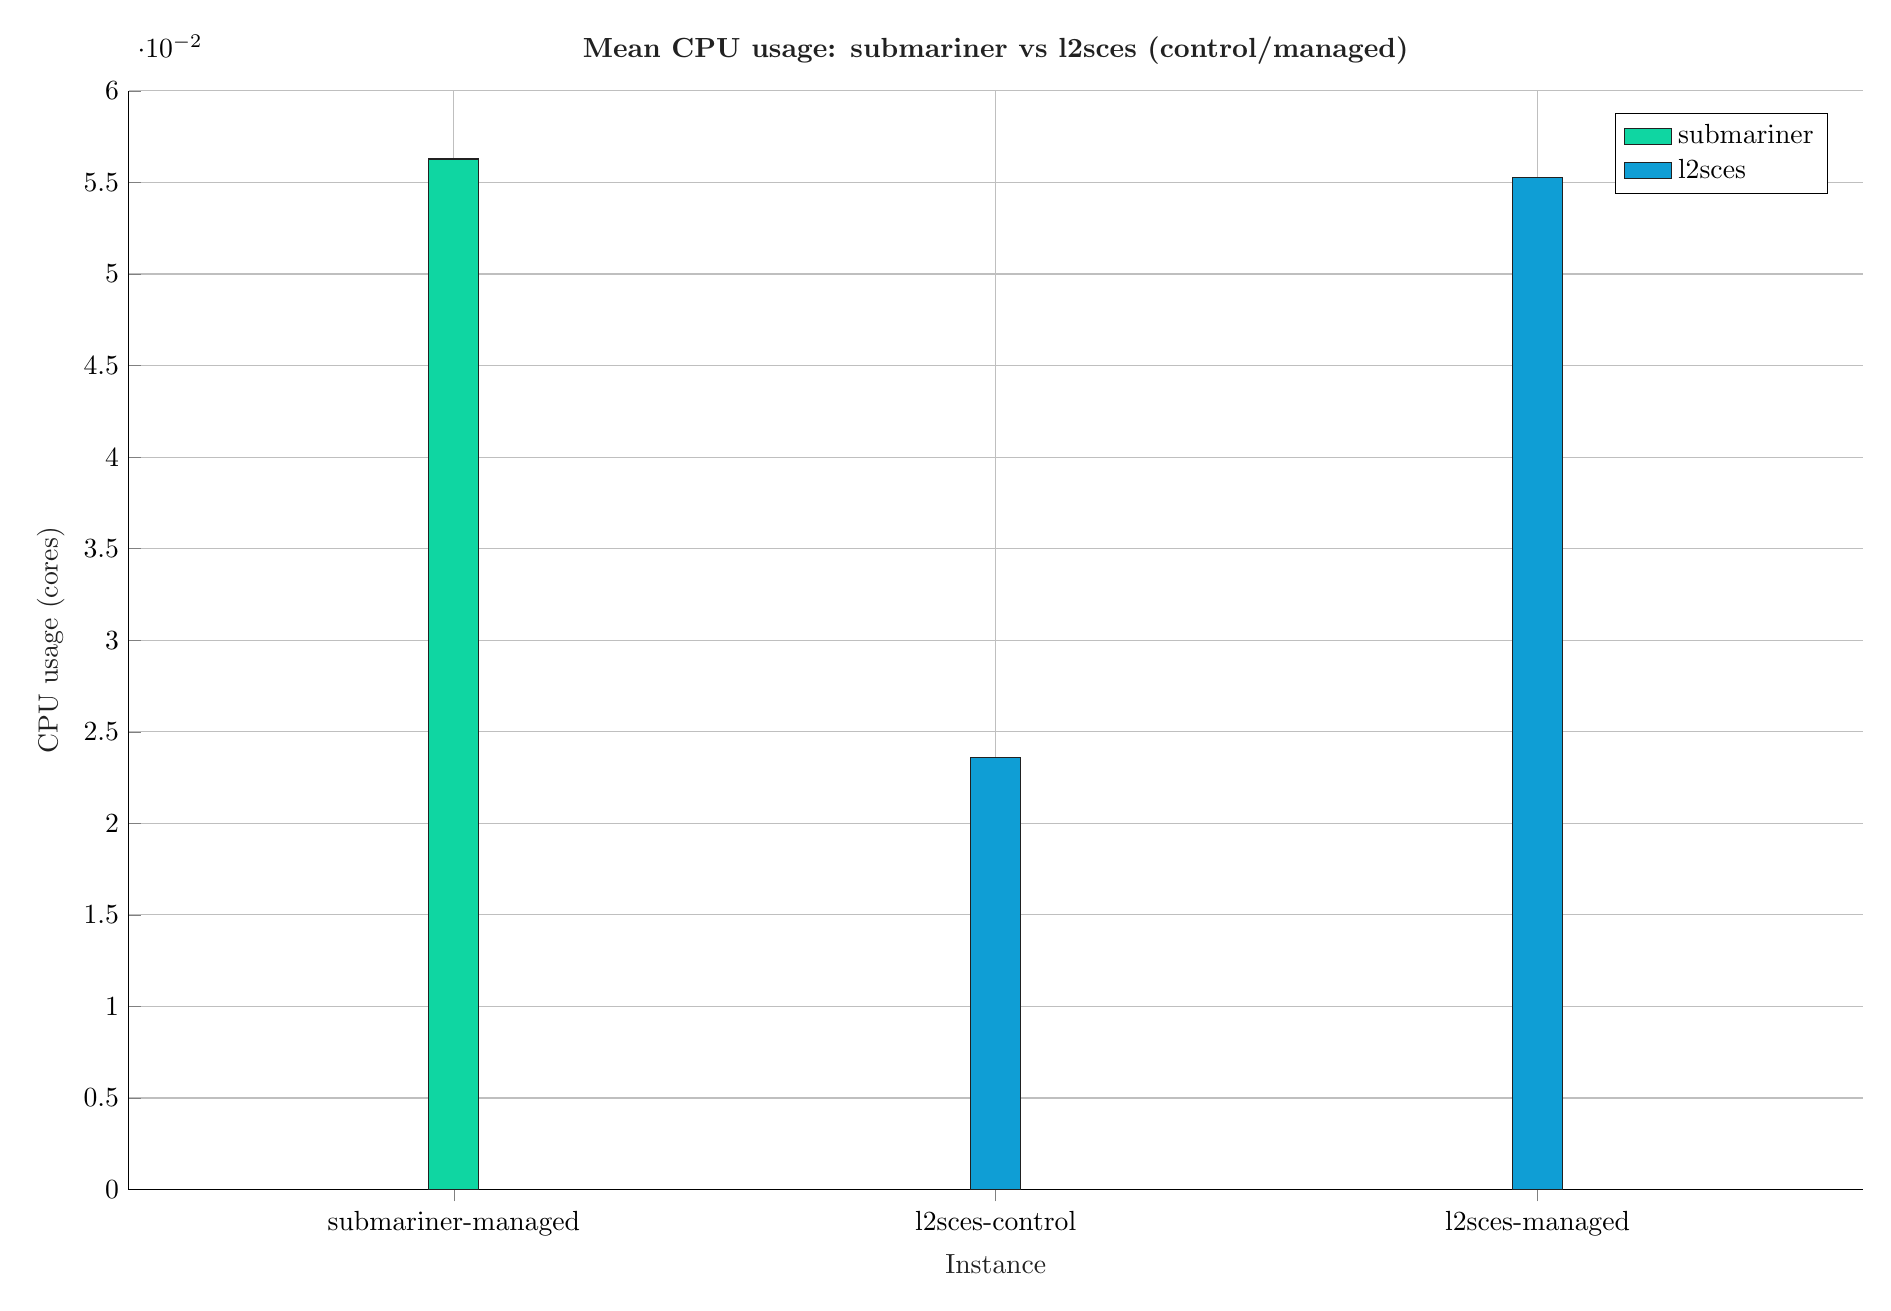
\begin{tikzpicture}

\begin{axis}[%
width=8.67in,
height=5.493in,
at={(1.454in,0.741in)},
scale only axis,
bar shift auto,
symbolic x coords={submariner-control,submariner-managed,l2sces-control,l2sces-managed},
enlarge x limits=0.2,
xtick=data,
xlabel style={font=\color{mycolor2}},
xlabel={Instance},
ymin=0,
ymax=0.06,
ylabel style={font=\color{mycolor2}},
ylabel={CPU usage (cores)},
axis background/.style={fill=white},
title style={font=\bfseries\color{mycolor2}},
title={Mean CPU usage: submariner vs l2sces (control/managed)},
axis x line*=bottom,
axis y line*=left,
xmajorgrids,
ymajorgrids,
legend style={legend cell align=left, align=left},
ybar,
bar width=18pt,
bar shift=0pt,
xtick={submariner-control,submariner-managed,l2sces-control,l2sces-managed},
enlarge x limits=0.3,
clip=false
]
\addplot[ybar, fill=mycolor1, draw=mycolor2, area legend] table[row sep=crcr] {%
submariner-control	0.00249921856213693\\
submariner-managed	0.056283422320178\\
l2sces-control	nan\\
l2sces-managed	nan\\
};
\addplot[forget plot, color=mycolor2] table[row sep=crcr] {%
submariner-control	0\\
l2sces-managed	0\\
};
\addlegendentry{submariner}

\addplot[ybar, fill=mycolor3, draw=mycolor2, area legend] table[row sep=crcr] {%
submariner-control	nan\\
submariner-managed	nan\\
l2sces-control	0.0235713020423083\\
l2sces-managed	0.0552811960047451\\
};
\addplot[forget plot, color=mycolor2] table[row sep=crcr] {%
submariner-control	0\\
l2sces-managed	0\\
};
\addlegendentry{l2sces}

\end{axis}
\end{tikzpicture}%